\section{Results}
\label{section:discussion&results:experiment-results}
TODO: Write introduction
% Dataset 1
\subsection{Dataset 1}
\import{./tables/results/dataset_1}{Average-metric-dataset-1.tex}
\begin{figure}[h!]
  \centering
  \begin{subfigure}[b]{0.49\textwidth}
    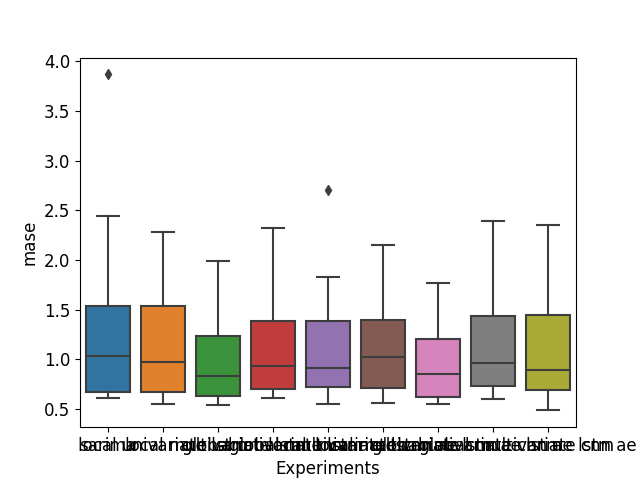
\includegraphics[width=\textwidth]{./figs/results/boxplot/mase-dataset_1.png}
    \hfill
    \caption{MASE boxplot of predictions made on dataset 1}
    \label{fig:results:boxplot-mase-dataset-1-mase}
  \end{subfigure}
  \begin{subfigure}[b]{0.49\textwidth}
    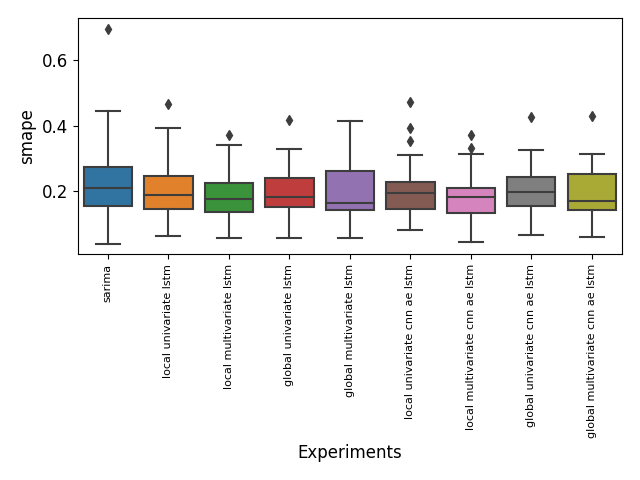
\includegraphics[width=\textwidth]{./figs/results/boxplot/smape-dataset_1.png}
    \hfill
    \caption{sMAPE boxplot of predictions made on dataset 1}
    \label{fig:results:boxplot-mase-dataset-1-smape}

  \end{subfigure}
\end{figure}
% \begin{figure}[h!]
%   \centering
%   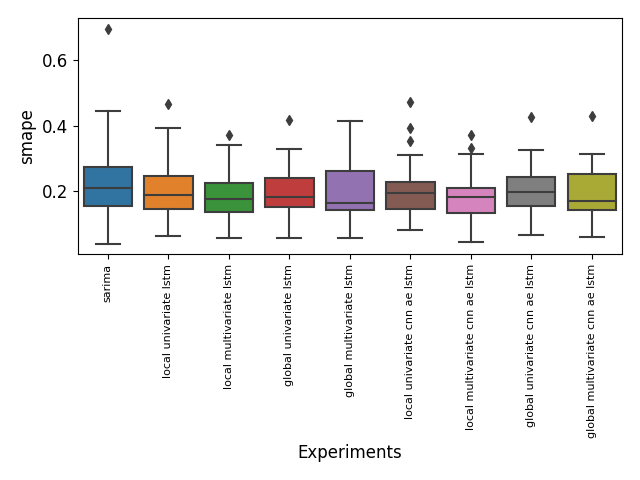
\includegraphics[width=\textwidth]{./figs/results/boxplot/smape-dataset_1.png}
%   \hfill
%   \caption{sMAPE boxplot of predictions made on dataset 1}
%   \label{fig:results:boxplot-mase-dataset-1-smape}
% \end{figure}

\Cref{table:Average-metric-dataset-1} shows the mean metrics accross
all the time series in dataset 1. The poorest perfoming model accross the board
is SARIMA, with a MASE of $1.294$, sMAPE of $0.239$ and 7 day MASE of $1.063$.
All the different LSTM structures and hybrid methods outperformed SARIMA.

The multivariate models outperformed all the their retrospective univariate counterpartners.
The global univariate LSTM outperforms the local univariate on both MASE and sMAPE,
but this results is not reproduced for the multivariate models, or the CNN-AE-LSTM models.

All the model structures perfoms slightly better with our proposed CNN-AE-LSTM method, except for
the global univariate CNN-AE-LSTM.

The most consistent models with the least amount of variance are the multivariate models.
The local multivariate CNN-AE-LSTM and the local multivariate LSTM were the only two models
who beat the naive 7-day prediction. The best performing model is the local multivariate CNN-AE-LSTM.

The mean MASE dataset across all models on dataset 1 is $0.971$,
the mean sMAPE is $0.2034$,
and the mean MASE 7-day is $0.9976$.


\subsection{Dataset 2}
% Dataset 2

\begin{samepage}
  \import{./tables/results/dataset_2}{Average-metric-dataset-2.tex}
  \begin{figure}[ht!]
    \centering
    \begin{subfigure}[b]{0.49\textwidth}
      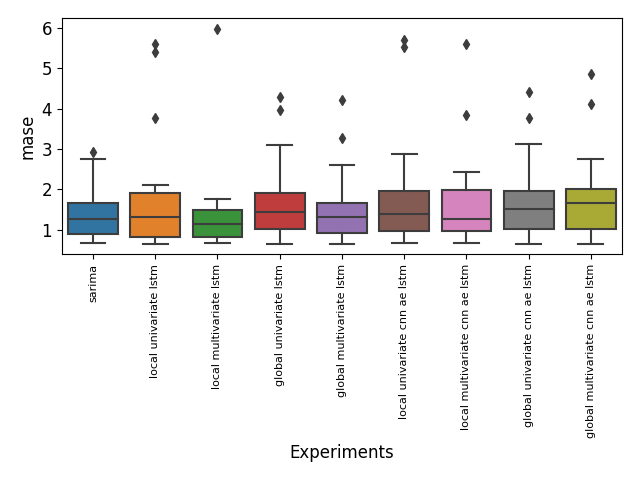
\includegraphics[width=\textwidth]{./figs/results/boxplot/mase-dataset_2.png}
      \hfill
      \caption{Boxplot of predictions made on dataset 2}
      \label{fig:results:boxplot-mase-dataset-2-mase}
    \end{subfigure}
    \begin{subfigure}[b]{0.49\textwidth}
      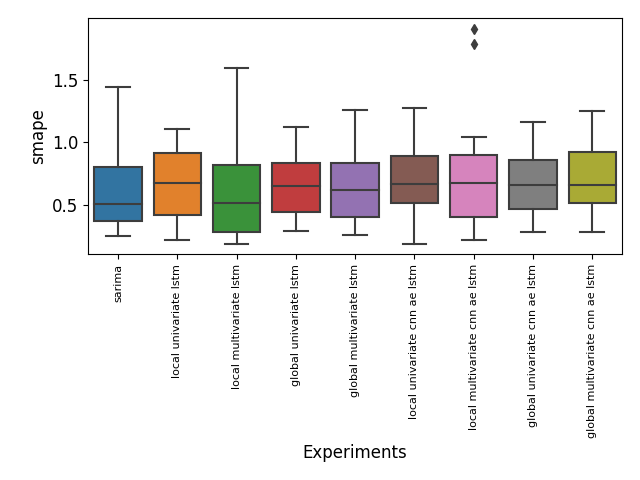
\includegraphics[width=\textwidth]{./figs/results/boxplot/smape-dataset_2.png}
      \hfill
      \caption{sMAPE boxplot of predictions made on dataset 2}
      \label{fig:results:boxplot-mase-dataset-2-smape}
    \end{subfigure}
  \end{figure}
\end{samepage}

Compared to dataset 1, dataset 2 proved to be a much more difficult dataset to forecast.
Compared to the NN models SARIMA performs a lot better, with a mase of $1.472$, a 7-day MASE of $0.707$ and smape of $0.633$.
Some of the results from dataset 1 are reproduced on dataset 2. For example the global univariate LSTM outperform
the local univariate LSTM. The multivariate models outperforms the univariate models.
On dataset 2 however all the CNN-AE-LSTM methods performs poorly compared to the LSTM models.
The best performing model on dataset 2 is local multivariate LSTM with a mase of $1.377$ a sMAPAE of $0.603$
and $0.697$.

The mean MASE across dataset 2 is $1.652$,
the mean sMAPE is $0.697$,
and the mean MASE 7-day is  $0.7306$.

% Dataset 3
\subsection{Dataset 3}
\begin{samepage}
  \import{./tables/results/dataset_seasonal}{Average-metric-dataset-seasonal.tex}
  \begin{figure}[h!]
    \centering
    \begin{subfigure}[b]{0.49\textwidth}
      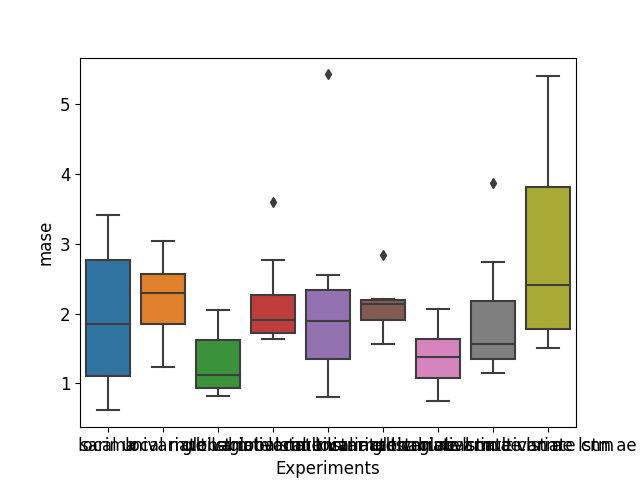
\includegraphics[width=\textwidth]{./figs/results/boxplot/mase-dataset_seasonal.png}
      \hfill
      \caption{Boxplot of predictions made on seasonal dataset}
      \label{fig:results:boxplot-mase-dataset-3}

    \end{subfigure}
    \begin{subfigure}[b]{0.49\textwidth}
      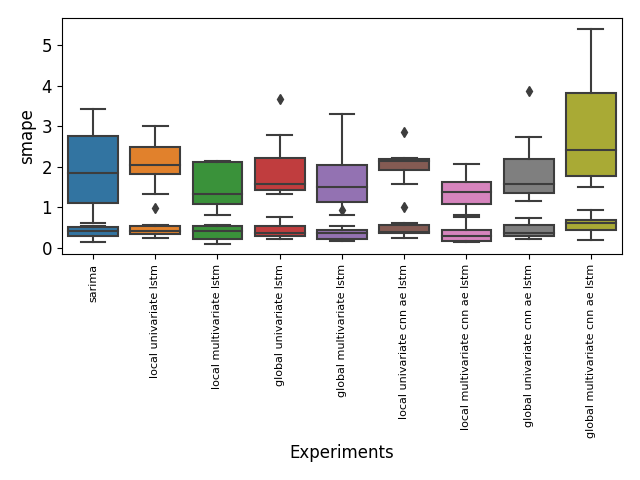
\includegraphics[width=\textwidth]{./figs/results/boxplot/smape-dataset_seasonal.png}
      \hfill
      \caption{Boxplot of predictions made on seasonal dataset}
      \label{fig:results:boxplot-smape-dataset-3}
    \end{subfigure}
  \end{figure}
\end{samepage}
On dataset 3 SARIMA, again, outperforms the purely local univariate LSTM baseline.
Many of the same patterns repeats on dataset 3 as with dataset 1 and 2, multivariate beats univariate,
global unviariate beats local univariate.
On dataset 3 it seems that the CNN-AE-LSTMs outperforms the LSTMs once again, except for the
best perfoming model, which is the local multivariate LSTM.


\todo[inline]{Update mean values! They are old}
The mean MASE for dataset 3 is $2.009$,
the mean sMAPE data set 3 is $0.4362$,
and the mean MASE 7-day is $1.131$.



% Globale modeller er dårligere på mase 7 bortsett fra.
% All results tables

\todo[inline]{Change name of dataset seasonal to dataset 3}
\todo[inline]{Update metric names to be MASE, sMAPE, MASE-7}


